\documentclass[12pt]{article}
\usepackage{latexsym,amssymb,amsmath} % for \Box, \mathbb, split, etc.
% \usepackage[]{showkeys} % shows label names
\usepackage{cite} % sorts citation numbers appropriately
\usepackage{path}
\usepackage{url}
\usepackage{verbatim}
\usepackage[pdftex]{graphicx}

% horizontal margins: 1.0 + 6.5 + 1.0 = 8.5
\setlength{\oddsidemargin}{0.0in}
\setlength{\textwidth}{6.5in}
% vertical margins: 1.0 + 9.0 + 1.0 = 11.0
\setlength{\topmargin}{0.0in}
\setlength{\headheight}{12pt}
\setlength{\headsep}{13pt}
\setlength{\textheight}{625pt}
\setlength{\footskip}{24pt}

\renewcommand{\textfraction}{0.10}
\renewcommand{\topfraction}{0.85}
\renewcommand{\bottomfraction}{0.85}
\renewcommand{\floatpagefraction}{0.90}

\makeatletter
\setlength{\arraycolsep}{2\p@} % make spaces around "=" in eqnarray smaller
\makeatother

% change equation, table, figure numbers to be counted inside a section:
\numberwithin{equation}{section}
\numberwithin{table}{section}
\numberwithin{figure}{section}

% begin of personal macros
\newcommand{\half}{{\textstyle \frac{1}{2}}}
\newcommand{\eps}{\varepsilon}
\newcommand{\myth}{\vartheta}
\newcommand{\myphi}{\varphi}

\newcommand{\IN}{\mathbb{N}}
\newcommand{\IZ}{\mathbb{Z}}
\newcommand{\IQ}{\mathbb{Q}}
\newcommand{\IR}{\mathbb{R}}
\newcommand{\IC}{\mathbb{C}}
\newcommand{\Real}[1]{\mathrm{Re}\left({#1}\right)}
\newcommand{\Imag}[1]{\mathrm{Im}\left({#1}\right)}

\newcommand{\norm}[2]{\|{#1}\|_{{}_{#2}}}
\newcommand{\abs}[1]{\left|{#1}\right|}
\newcommand{\ip}[2]{\left\langle {#1}, {#2} \right\rangle}
\newcommand{\der}[2]{\frac{\partial {#1}}{\partial {#2}}}
\newcommand{\dder}[2]{\frac{\partial^2 {#1}}{\partial {#2}^2}}

\newcommand{\nn}{\mathbf{n}}
\newcommand{\xx}{\mathbf{x}}
\newcommand{\uu}{\mathbf{u}}

\newcommand{\junk}[1]{{}}

% set two lengths for the includegraphics commands used to import the plots:
\newlength{\fwtwo} \setlength{\fwtwo}{0.45\textwidth}
% end of personal macros

\begin{document}
\DeclareGraphicsExtensions{.jpg}

\begin{center}
\textbf{\Large Template for Technical Reports} \\[6pt]
  Matthias K. Gobbert \\[6pt]
  Department of Mathematics and Statistics,
  University of Maryland, Baltimore County  \\[6pt]
  gobbert@umbc.edu, \url{www.math.umbc.edu/~gobbert}
\end{center}

\begin{abstract}
The abstract should be a succinct summary of your topic and your solution.
It should characterize what this
report contains including the relevant conclusion from the results presented.
Since abstracts are often entered in searchable databases,
use only English words, no
formulas, no citations, no references to any formula in your text,
etc. Its length is often restricted, e.g., to 100 or 200~words.
\end{abstract}

\subparagraph{Key words.} Provide five key words or phrases that
describe your topic, methods, and results.

\subparagraph{AMS subject classifications (2010).}
Provide up to five subject classification codes here;
search for the string ``MSC'' at \url"www.ams.org".

\section{Introduction}

\subsection{Some Technicalities}

Where to find this document? You may very well wonder about this point,
if this document was given to you in paper form; if you downloaded it
from my homepage, this will be obvious, of course. This document is
available in the \LaTeX\ area of my homepage, which I will refer to
as \cite{homepage} in the following.
You will need to download several files, namely
\verb+template.tex+, \verb+template.bib+, the three figures
\verb+figconvrateloglog.jpg+, \verb+figconvrateplot.jpg+,
and \verb+mesh_solution.jpg+, and the Matlab code \verb+plot_loglog.m+.

How to read this document? Reading the resulting printout is useful,
but you must also study carefully the \LaTeX-source code;
I am trying to use all sorts of examples of sophisticated features.
Notice how the result has a very simple appearance about it, but it takes
some correct use of \LaTeX\ to achieve this goal at times.
When reading the source code, pay particular attention, how all the
referencing is done using the commands \verb+\label+ to set the label
and \verb+\ref+ to refer to it. There are no separate labels or references
for figures, tables, equations, sections, rather the meaning of the
\verb+\label+ command is determined from the context, in which it appears.
I have adopted the scheme to use the first three letters of the
key for each label to indicate to myself, what kind of an object it
refers to, so I use `fig' for figure labels, `tab' for table labels, etc.;
see the source code.
% TMP
% How to create a printout of this document, though?
% See Section~\ref{sec:references} below.

\subsection{Philosophy of this Document}

This file is designed to show by
example, how some relevant features of \LaTeX\ can be used to put
together a technical report or a manuscript
in such a form that it can be submitted to a journal.
Any journal will have to work through your submission anyway, so
it makes no sense to try to deal with some of the more technical
requirements they have. Rather, your goal should be to provide clean
\LaTeX, so that the copy editor only has to work on the formalities,
but not the contents of the paper. In this spirit, it is very important
that you provide information in expected places in some expected
format; then the work of any editor is made easy. To this end, I
am also trying to use clean but basic \LaTeX2$_\varepsilon$;
this means that I am trying not
to use any fancy features like redefining section headings,
etc., but I allow myself the use of popular extensions that
are available in packages that come with the standard distribution
of \LaTeX\ under Linux.
Again, if a journal wants the paper to look different,
they will take care of that by using their macros.

The additional purpose of this document is to demonstrate some of
those more advanced of features of \LaTeX\ that are typically needed
like importing figures or creating reference lists. For more basic
commands, please see my basic sample document \emph{Some \LaTeX\ Introduction}
\cite{homepage}; here and throughout, pay attention to my citations,
as they are meant to show examples of how to cite certain types of
publications. For more information about \LaTeX, you should consider
\cite{Goossens94,Graetzer1996,Lamport94}.
Leslie Lamport is the original creator of \LaTeX,
and his book \cite{Lamport94}
should be the starting point, in particular its Chapters~1 through~3
\cite[Chapters~1--3]{Lamport94}.
The other books \cite{Goossens94,Graetzer1996}
are only needed for advanced uses of \LaTeX.
Both books have similar content overall,
but they have different approaches: \cite{Goossens94} is `horizontal'
and discusses material organized by package; I suggest to use it,
if you want to dig into the innards
of \LaTeX\ like redefining section headers or advanced float placement.
Compared to that, \cite{Graetzer1996} is organized `vertically,'
because it discusses tools for one topic from all available sources together.
If you need to typeset very complicted formulas or have other problems
with the mathematics, I recommend \cite{Graetzer1996} because of its
well-chosen examples and its organization.

For an excellent discussion of writing mathematics in general, let me point
to \cite{Higham98}. It contains more than the title lets on, namely
also very relevant remarks on the politics of publishing in
mathematics. If you are a Ph.D. student, you should definitely
read this book.

\section{Importing of Figures} \label{sec:import}

Notice carefully the use of \LaTeX's powerful capabilities for automatic
cross-referencing demonstrated
for equations, tables, and figures
in the following subsection,
Subsection~\ref{subsec:example}.

\subsection{Example} \label{subsec:example}

We know that the error of the finite difference approximation using
\begin{figure} \centering
  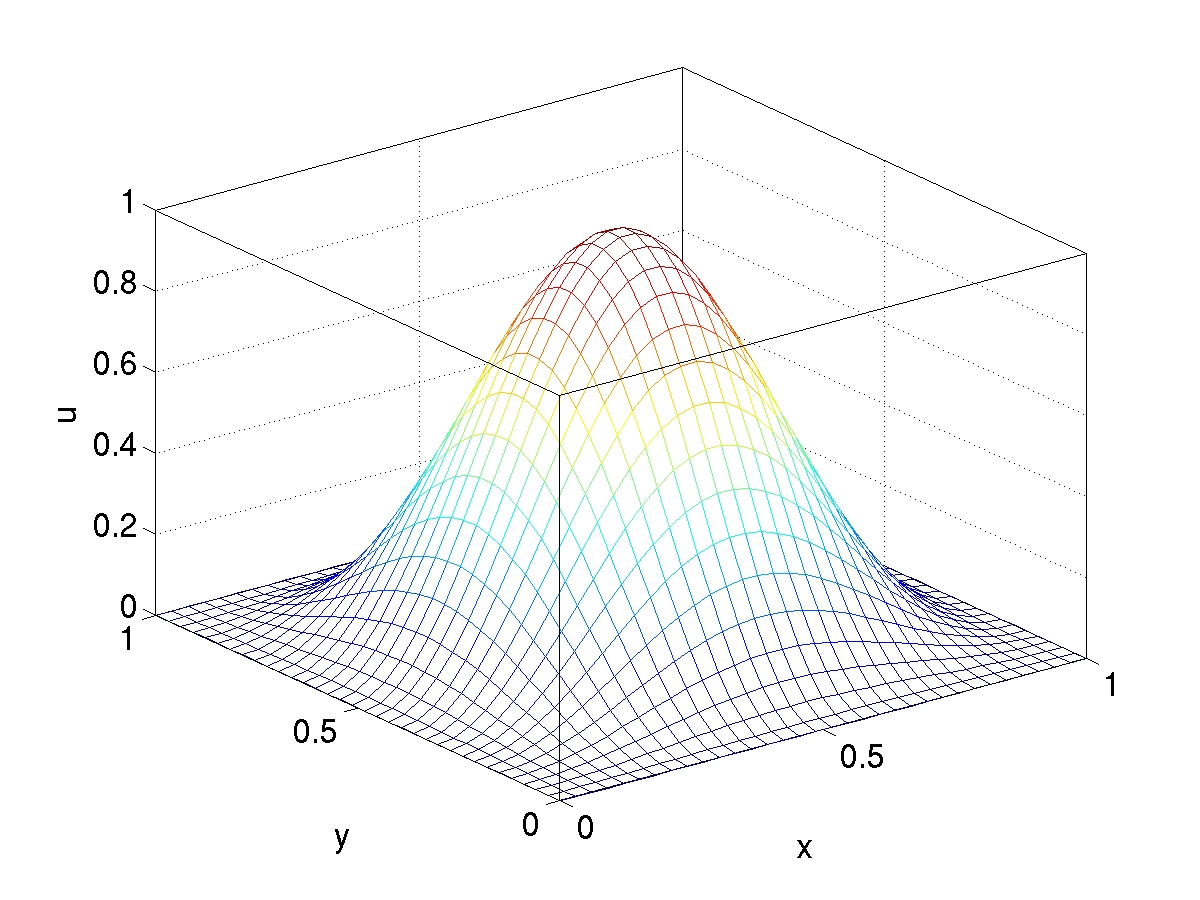
\includegraphics[width=0.5\textwidth]{mesh_solution}
  \caption{Solution to test problem with $h = 1 / 32$.}
  \label{fig:solplot}
\end{figure}
centered differences for an elliptic partial differential equation
satisfies
\begin{equation} \label{equ:convratequad}
  \norm{u - u_h}{\infty} = C h^2 \quad \mbox{as $h \rightarrow 0$},
\end{equation}
where $h$ denotes the maximum mesh spacing and
$C$ denotes a constant independent of $h$.
This can be demonstrated numerically by solving a problem with
a known solution $u$ like the test problem in \cite{RaimGobbert2010Poisson}.
First of all,
Figure~\ref{fig:solplot} shows the solution of the test problem obtained with
a mesh size of $h = 1 / 32$.
The convergence rate is displayed
\begin{table} \centering
  \caption{Demonstration of quadratic convergence rate for the test problem.}
  \label{tab:convdemo}
  \vspace{0.5\baselineskip}
  \begin{tabular}{rcccc}
    \hline
    $1 / h$ & $h$ & $\norm{u - u_h}{\infty}$ &
      $\frac{\norm{u - u_{2h}}{\infty}}{\norm{u - u_h}{\infty}}$ &
      $\frac{\norm{u - u_h}{\infty}}{h^2}$ \\
    \hline
       32 &   3.1250e-02 & 3.2189e-03 &   N/A  & 3.2962 \\
       64 &   1.5625e-02 & 8.0356e-04 & 4.0058 & 3.2914 \\
      128 &   7.8125e-03 & 2.0081e-04 & 4.0016 & 3.2901 \\
      256 &   3.9062e-03 & 5.0191e-05 & 4.0009 & 3.2893 \\
      512 &   1.9531e-03 & 1.2543e-05 & 4.0015 & 3.2881 \\
     1024 &   9.7656e-04 & 3.1327e-06 & 4.0039 & 3.2849 \\
     2048 &   4.8828e-04 & 7.8097e-07 & 4.0113 & 3.2756 \\
     4096 &   2.4414e-04 & 1.9356e-07 & 4.0348 & 3.2474 \\
     8192 &   1.2207e-04 & 4.6817e-08 & 4.1344 & 3.1418 \\
    16384 &   6.1035e-05 & 8.0469e-09 & 5.8180 & 2.1601 \\
    32768 &   3.0518e-05 & 2.9562e-09 & 2.7220 & 3.1742 \\
    \hline
  \end{tabular}
\end{table}
in table form as in Table~\ref{tab:convdemo}. We see that the error
decreases by a factor of $4$ for each halving of the mesh size.
Moreover, it is shown that $\norm{u - u_h}{\infty}$ divided by $h^2$
tends to a constant value, which is $C$ in (\ref{equ:convratequad}).

The same can be demonstrated in graphical form. It is conventional
to present the result in the form of a log-log plot.
Figure~\ref{fig:convrateab}~(a) shows this using Matlab's \verb+loglog+
function on the values of $1 / h$ and $\norm{u - u_h}{\infty}$.
What are we looking for? The answer is the slope of the almost linear
curve, and here is why: If we take the logarithm on both sides of
(\ref{equ:convratequad}), we obtain
\begin{displaymath}
  \log_{10}\left(\norm{u - u_h}{\infty}\right)
    = \log_{10}\left(C h^2\right)
    = \log_{10}\left(C\right) + \log_{10}\left(h^2\right).
\end{displaymath}
Using more rules for logarithms, this can be written as
\begin{equation} \label{equ:linearity}
  \log_{10}\left(\norm{u - u_h}{\infty}\right) =
    -2 \, \log_{10}\left({\textstyle \frac{1}{h}}\right)
    + \log_{10}\left(C\right),
\end{equation}
which demonstrates that $\log_{10} (\norm{u - u_h}{\infty})$ is
a linear function of $\log_{10} (1/h)$ with a slope of $-2$.
This is clearly demonstrated in Figure~\ref{fig:convrateab}~(b),
which also shows a linear approximation to the data as a dashed line.
\begin{figure} \centering
  \begin{tabular}{cc}
    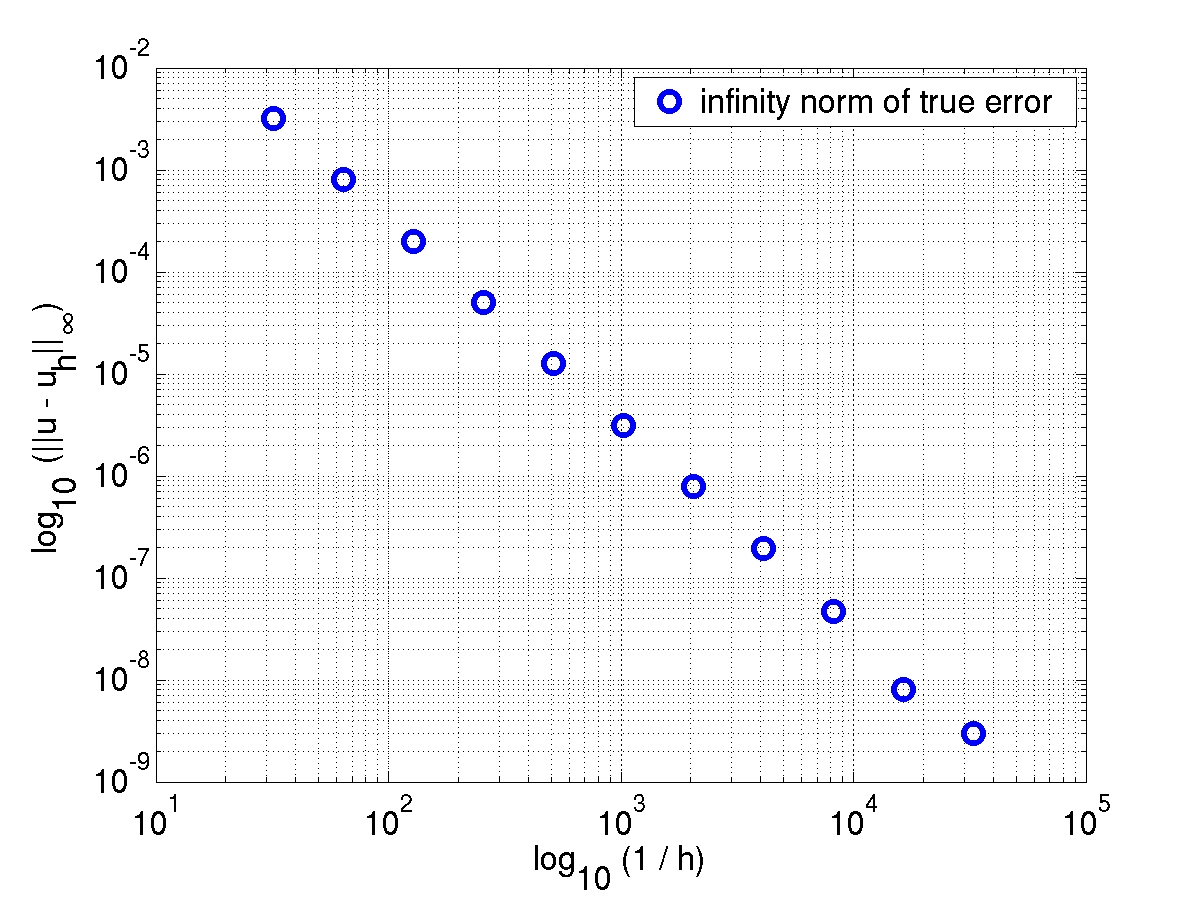
\includegraphics[width=\fwtwo]{figconvrateloglog} &
    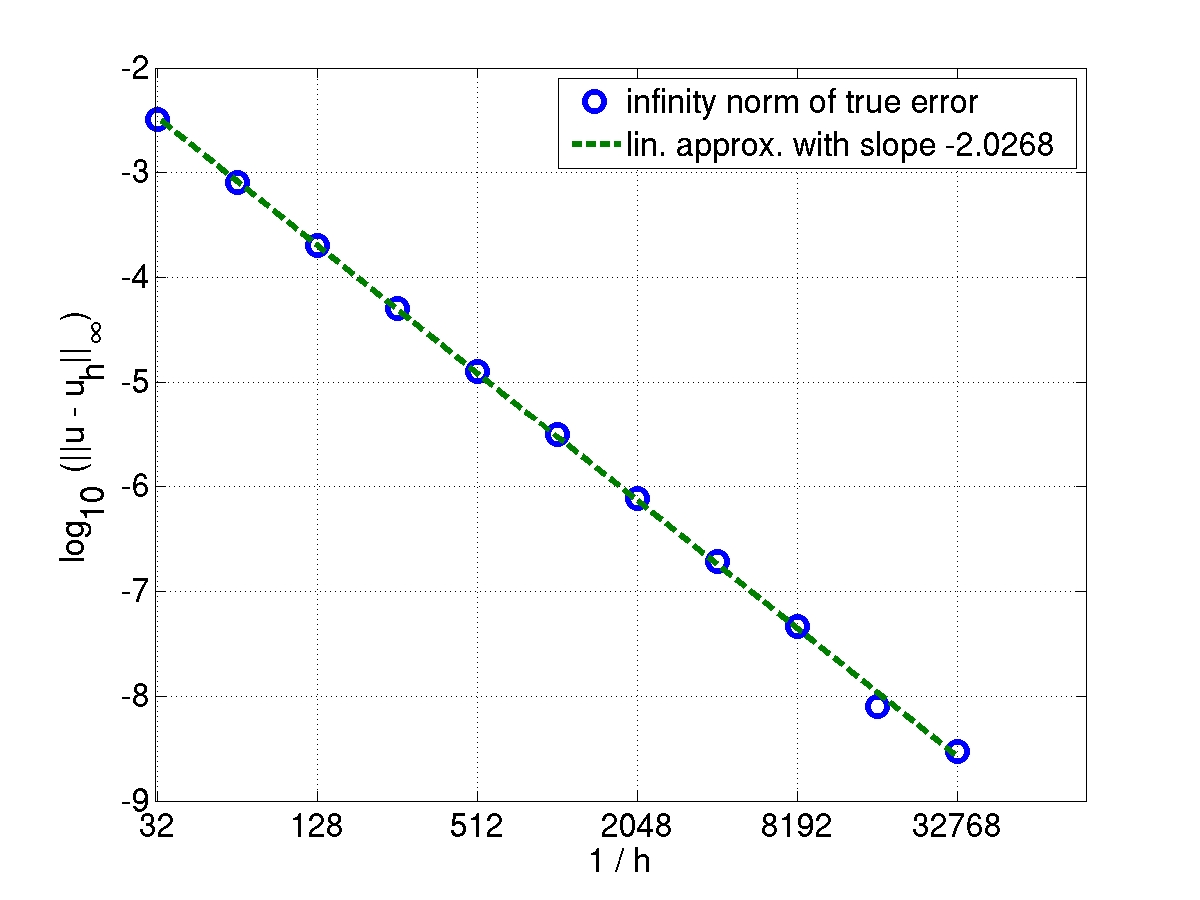
\includegraphics[width=\fwtwo]{figconvrateplot} \\
    (a) & (b)
  \end{tabular}
  \caption{Plot of true error of finite difference approximation,
  (a) using log-log plot, (b) using plot of the logarithm of the data;
  a linear approximation is included to demonstrate the linearity
  derived in (\ref{equ:linearity}); in turn, this equation reference
  is included in this caption to demonstrate that you need to process
  the tex file three times for this equation reference to be correct.}
  \label{fig:convrateab}
\end{figure}

\subsection{Some Comments}

This subsection is here mainly to demonstrate the use of a subsection.
This is likely appropriate in your section on Results, because you should
try to split those up into more manageable parts.

See the \LaTeX-code of this file for the code used to import the figures;
the Matlab code used to produce them is included as Appendix~\ref{app:code}.
You will likely not have any space in your report to include actual code, but
I wanted to demonstrate the use of an appendix, and that was a good purpose;
you also may be able to learn some Matlab from it, if you wish to.

Basically, the importing of postscript files is done using the
\verb+\includegraphics+ command from the \verb+graphicx+ package;
this package is loaded at the beginning of this file by
the \verb+\usepackage{graphicx}+ command.
It is not strictly part of \LaTeX2$_\varepsilon$,
however, the \verb+graphicx+ package \emph{is}
part of the ``standard distribution of \LaTeX2$_\varepsilon$,'' so it is
okay (i.e., portable) to use it. (By the way, this ``standard distribution''
is included with any installation of Linux.)

Now, concretely, the \verb+\includegraphics+ command accepts the name of
the file to be imported as required argument (in the curly braces).
It probably has a default for the size of the imported figure, but you
should really control this yourself manually.
That can be done by using the \verb+height=+ or
\verb+width=+ flags in the optional argument (in the brackets);
you should only give one of them, so that the
figure gets scaled proportionally in both directions,
that is, without changing its aspect ratio.
Here is how Figure~\ref{fig:solplot} was coded:
\begin{verbatim}
\begin{figure} \centering
  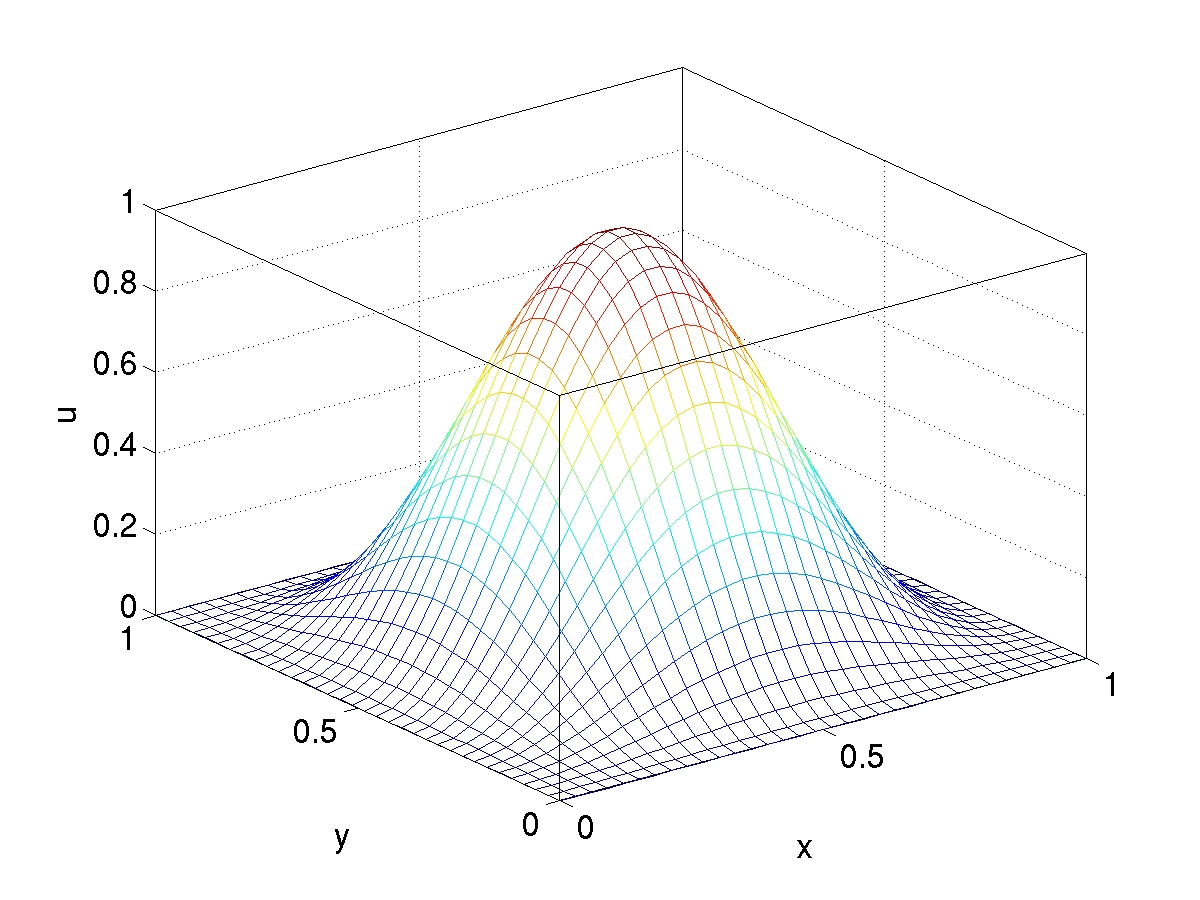
\includegraphics[width=0.5\textwidth]{mesh_solution}
  \caption{Solution to test problem with $h = 1 / 32$.}
  \label{fig:solplot}
\end{figure}
\end{verbatim}
It is best to express your width relative to the \verb+\textwidth+ length.
If you have multiple figures whose width should all be the same,
you can define a length; see the \LaTeX-code for the use
of \verb+\fwtwo+ in Figure~\ref{fig:convrateab}.
The \verb+caption+ creates the caption, and the \verb+label+ sets the
label that I am referring to here; please read the source code of this file.
You will notice that I am referring to the file \verb+mesh_solution.jpg+
without giving its extension \verb+jpg+. That is possible because of the
\verb+\DeclareGraphicsExtensions{.jpg}+ command immediately after the
\verb+\begin{document}+ command.
If you wish
to overwrite its effect, you can always do this by supplying a full
file name to the \verb+\includegraphics+ command.

A final word on placement of figures and tables: Remember that they are
floats, a technical term for a text object that is floated about to fit
it in a visually pleasing way as opposed to putting it right in order of
the text. The placement of them is perennially a problem, in particular if
you have many of them. The best suggestion I have is to resize them
reasonably small so that several can fit on one page. That gives \LaTeX\
the most flexibility in placing them. To be complete, placement of floats
is controlled by a number of proportional variables like the fraction of
a page that can be a float, the fraction of space at top that can be occupied
by one, the fraction of space at the bottom that can, etc. If you want
to learn about that, I recommend \cite{Goossens94}, but a general
introduction is contained in \cite{Lamport94}.

\section{References} \label{sec:references}

For anyone serious about writing more than a single document, I urge
the use of the \textsc{Bib}\TeX\ bibliography system. Its complete
reference can be found in \cite[Appendix B]{Lamport94}.
In fact, even for a single document, it makes already sense to use it.
Let me explain both points presently.

\textsc{Bib}\TeX\ is really a bibliography database system. Your whole
bibliography is contained in one or several files, in this case the file
\verb+template.bib+. In your text, you use then the \verb+\cite+ command
on the keys of those references. The point is that only those references
that you actually use get included in the references (note that for
instance the reference \verb+Gobbertiwce+ appears in the \verb+bib+-file
but not in the bibliography). To accomplish this,
you must run \LaTeX\ once to put all requested references in the
\verb+template.aux+, then run \textsc{Bib}\TeX\ once to pick up the
bibliographical information and create the file \verb+template.bbl+,
which contains the formated bibliography. Finally, you must run \LaTeX\
\emph{twice}: At first, it includes the bibliography in your document,
but during this first pass, it cannot have set the reference labels,
so in the second pass, the labels are correctly set. The upshot is,
always run \LaTeX\ twice to get all cross-referencing right. Remember
that this is needed whenever \emph{any} label or reference changes.
In summary, you should issue these commands:
\begin{verbatim}
  pdflatex template
  bibtex template
  pdflatex template
  pdflatex template
\end{verbatim}
Notice how \verb+plflatex+ is run \emph{twice} to get the cross-references
right. That is misleading, though, because you actually need to run
it \emph{three} times in total for this document
(which is done implicitly in the list above!),
if you want to get the formula reference right that appears in the caption
of Figure~\ref{fig:convrateab}.

All this is started by the \verb+\bibliography{template}+ command
at the far end of this file; here, \verb+template+ refers to the file
\verb+template.bib+. Now, this is really a little unrealistic, because
the main advantage of \textsc{Bib}\TeX\ is that you can use one
\verb+bib+-file for all your research (or one per research project)
and maintain them at a central location. So, it is just done this way
here, so that you can download one simple file instead of my whole
bibliography database. Really, the following is my usual full command:
\begin{verbatim}
  \bibliography{/home/gobbert/soft/tex/biblio/curr/mgenmath,%
                /home/gobbert/soft/tex/biblio/curr/mreschem,%
                /home/gobbert/soft/tex/biblio/curr/mresmath,%
                /home/gobbert/soft/tex/biblio/curr/mresboltz}
\end{verbatim}
Actually, even this one is shortened to include only those \verb+bib+-files
related to that particular paper; I have more such files with bibliographical
information on other research projects.

What are the advantages of using \textsc{Bib}\TeX? I personally find
it actually easier to enter the information, hence I would even use it
for a single document. When entering it, I do not have to worry about the
referencing style required by the particular journal. Rather, \textsc{Bib}\TeX\
worries about that, when writing the \verb+bbl+-file. This appearance
is controlled by the \verb+\bibliographystyle{siam}+ command, where I
have chosen the referencing style for SIAM journals, which is one of
the standard ones supplied. So, here is the second advantage: You can
change the appearance of your bibliography merely by changing the
argument of the \verb+\bibliographystyle+ command. You may want to try
some other default ones like \verb+plain+ (which is pretty plain but elegant)
or \verb+ieeetr+ (which is quite nice).
Many journals supply their own bibliography style files,
such as \verb+nature+ or \verb+science+,
which you might need to download, since they are not part of the
standard distribution of \LaTeX.

Notice finally that the data in \verb+bib+-file(s) should be sensibly
arranged, for instance, alphabetically by the last name of the first
author; this order does not impact the order of appearance in your
document. A note on order might be in order: In engineering, you
often quote references by order of appearance, as you will see when
using \verb+ieeetr+. In mathematics, it is conventional to alphabetize
references by the last names of all authors, as is done by \verb+siam+.
Notice, how \cite{GoPr1} appears before \cite{Gobbert} independent of
chronology, but rather based on the last name of the second author.
(In fact, the order of the joint papers with Andreas Prohl is based on
alphabetizing the titles, which is quite non-sensical; if I did this
by hand, I would choose a chronological order.)

Other technical things include that several references together should
be referred to in one \verb+\cite+ command, namely as
\cite{Goossens94,Graetzer1996,Lamport94} and not as three citations
\cite{Goossens94}, \cite{Graetzer1996}, and \cite{Lamport94}.
Notice also that it does not matter if I say
\cite{Goossens94,Graetzer1996,Lamport94},
\cite{Graetzer1996,Goossens94,Lamport94}, or
\cite{Lamport94,Goossens94,Graetzer1996}, etc.;
see the source code to understand the difference between these
three citations!
That is accomplished by using the package \verb+cite+.
Notice that \verb+cite+ does some quite amazing things:
For instance, here are all publications cited in this template
that involve actual science (as opposed to \LaTeX\ and the like)
\cite{Gobbert,GoPr1,GoPr2,Gobbertima2000,Gobbertsiap2000,Ho95,Iserles96,RaimGobbert2010Poisson,Sharmathesis2010};
notice how \verb+cite+ groups the references without my doing
anything special; see the source code.

You might have noticed that the bibliography style \verb+siam+
uses all lowercase letters for the titles of articles.
That is not appropriate for proper names of software, places, or
natural persons that include Capital letters. In such cases,
you must inform \textsc{Bib}\TeX\ of these situations by putting
braces around either the letter or the word in question; see
\cite{Gobbertsiap2000} for an example.
It is also possible in the \verb+bib+-file to give \LaTeX\ commands like
\verb+\-+ to inform it of places for allowable hyphenation in a word that
it could not find by itself. That was done for the publisher of
\cite{Graetzer1996}.
% ; try processing this file without the \verb+\-+
% and you will get an \verb+Underfull \hbox+ warning.

I wanted to provide examples for the most common citations here.
So, for instance, \cite{Gobbertsiap2000} is the citation of a paper that
has been \emph{submitted} for publication. After acceptance, I would list
it as \emph{accepted} like \cite{Gobbertiwce}.
Finally, after I have received the page proofs,
I would list the paper as being \emph{in press} like \cite{Gobbertjcp2004}.
(By the way, these papers are used as dummies here; they will remain
listed as submitted, accpeted, and in press in this template,
even once they appear.) On the other
hand, \cite{GoPr1} has appeared and shows all relevant information for
a journal article. For a book that appeared in a series,
\cite{Iserles96} would be an example (notice that this
one does not have a volume number in that series).
\cite{Sharmathesis2010} is the example of a M.S. thesis completed at UMBC,
and \cite{RaimGobbert2010Poisson} is a technical report.

Finally, let me discuss one kind of reference that causes regular
confusion on how to use correctly, namely the ``private'' or ``personal
communications.''
\cite{Ho95} is an example of how I have used this category in the past myself;
the point was that we used chemical formulas that were only
available to us as copy of transparencies. A more typical application
would be, if you have an e-mail exchange with a famous and distant researcher
as I am characterizing in \cite{BigShot}. I hope this helps to clear
up some confusion on the issue. If in doubt, ask your advisor for advice.

\section{Conclusions}

Finally, let me say that this document was put together with quite a bit
of thought over some time, but I probably still forgot a number of very
important features that you will need. In doubt, read the original
documentation \cite{Lamport94}, in particular its Chapters~1 through~3.

\section*{Acknowledgments}

This section is not numbered, because it is an optional add-on to the
paper and not directly related to its contents.
Acknowledgments for two kinds of support are customary here, namely
financial and scientific support: You would list the
support of a funding agency or grant here including the grant number.
And you can thank others for useful discussion or kind support or
something similar. For instance, you will be the only author of your
project report (contrary to a joint paper), but your advisor or
someone else may provide substantial support to the completion of
this work; you should acknowledge that person here. On the other hand,
if I as instructor provide mainly technical and organizational support,
that does not warrant a mention here.
Notice that if you are funded by a grant, you should ask the PI
to suggest an offical phraseology of the acknowledgment.
 
\appendix

\section{Code for Convergence Rate Plots} \label{app:code}

Here is an example of an appendix and of how to do it in \LaTeX.
The command \verb+\appendix+ is the key, because it switches the
counting to Capital letters instead of numbers. Then, continue to
use \verb+\section+ and \verb+\subsection+ as usually.

\verbatiminput{plot_loglog.m}

\bibliographystyle{siam}
\bibliography{template}

\end{document}

